\documentclass[border=0pt,10pt]{standalone}
\usepackage[T1]{fontenc}
\usepackage{lmodern}
\usepackage{pgfplots}
\pgfplotsset{compat=1.17}
\usepgfplotslibrary{groupplots}
\usepackage{xcolor}
\definecolor{oi-blue}{HTML}{0072B2}
\definecolor{oi-vermillion}{HTML}{D55E00}
\definecolor{oi-green}{HTML}{009E73}
\definecolor{oi-purple}{HTML}{CC79A7}
\definecolor{oi-black}{HTML}{000000}
% semantic_sha256: bd2a953e6fdeba82f892112e77e569b479863bd0d1672a21f119ca1f80c333bc
\begin{document}
\begin{minipage}{181.86mm}
\centering
{\bfseries\fontsize{10}{12}\selectfont PP-U-ARPLS | D2 | final\_refit}\\[2mm]
{\fontsize{8}{10}\selectfont planned=33, monitored=33, missing-history=0, status=complete\_history\_coverage}\\[3mm]
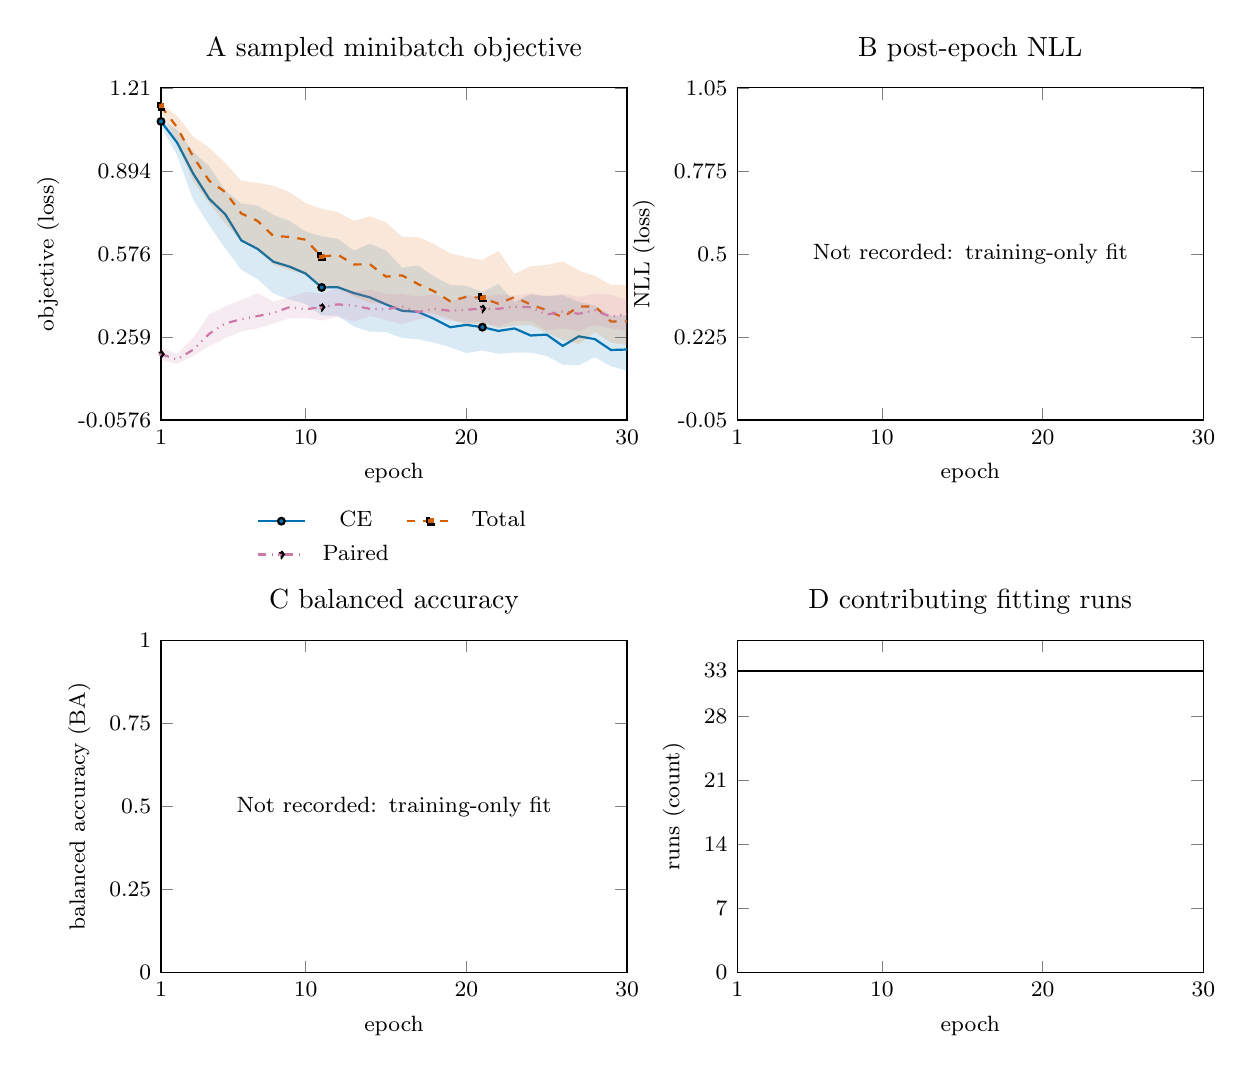
\begin{tikzpicture}
\begin{groupplot}[group style={group size=2 by 2, horizontal sep=14mm, vertical sep=28mm}]
\nextgroupplot[width=75mm, height=58mm, title={A sampled minibatch objective}, xlabel={epoch}, ylabel={objective (loss)}, xmin=1, xmax=30, xtick={1,10,20,30}, ymin=-0.057645774781703955, ymax=1.2105612704157829, ytick={-0.057645774781703955,0.25940598651766772,0.5764577478170394,0.89350950911641103,1.2105612704157829}, yticklabels={-0.0576,0.259,0.576,0.894,1.21}, tick label style={font=\fontsize{8}{9}\selectfont, text=black}, label style={font=\fontsize{8}{9}\selectfont, text=black}, title style={font=\fontsize{10}{11}\selectfont, text=black}, legend style={at={(0.5,-0.24)},anchor=north,draw=none,fill=none,font=\fontsize{8}{9}\selectfont,row sep=1pt,column sep=4pt,legend columns=2}]
\addplot[fill=oi-blue,opacity=0.15,draw=none,forget plot] coordinates {(1,1.0629354774951936) (2,0.95326906144618984) (3,0.7836405485868454) (4,0.68607073724269863) (5,0.59761036634445186) (6,0.51596058905124664) (7,0.48146395683288573) (8,0.42513887882232665) (9,0.40300215035676956) (10,0.38574503213167188) (11,0.34207277446985246) (12,0.34040363579988481) (13,0.299332794547081) (14,0.27989394366741183) (15,0.27878197208046912) (16,0.25552180036902428) (17,0.25092809498310087) (18,0.23773119449615479) (19,0.2205686628818512) (20,0.19817625731229782) (21,0.20815695449709892) (22,0.19510200992226601) (23,0.20034355893731118) (24,0.19935705065727233) (25,0.1871510200202465) (26,0.1540608935058117) (27,0.15137918554246427) (28,0.18213469684123992) (29,0.14746512621641159) (30,0.1312257494777441) (30,0.34274543821811676) (29,0.33978441208600996) (28,0.37955868095159534) (27,0.39352489113807682) (26,0.41905250251293186) (25,0.4143721327185631) (24,0.42229958325624467) (23,0.39287456423044204) (22,0.46193255782127379) (21,0.43138385862112044) (20,0.45463284403085708) (19,0.45804625600576399) (18,0.49030521512031555) (17,0.53223904073238371) (16,0.52431598007678981) (15,0.58932197690010069) (14,0.61515409648418429) (13,0.58907542526721957) (12,0.63414781391620634) (11,0.64380972385406499) (10,0.66187095642089844) (9,0.70276533663272855) (8,0.72540526986122134) (7,0.76101464033126831) (6,0.7690923660993576) (5,0.81883160471916194) (4,0.91146737039089198) (3,0.96603077352046962) (2,1.0506119191646577) (1,1.0918724119663239)};
\addplot[color=oi-blue, mark=*, mark options={draw=black}, mark repeat=10, mark size=1.2pt, solid, line width=0.8pt] coordinates {(1,1.0825216174125671) (2,1.0020235329866409) (3,0.88371138274669647) (4,0.7872515469789505) (5,0.72778388857841492) (6,0.62808592617511749) (7,0.59618464112281799) (8,0.54662413895130157) (9,0.52814677357673645) (10,0.50172161310911179) (11,0.44861067831516266) (12,0.44947529584169388) (13,0.42712313681840897) (14,0.41058198362588882) (15,0.38391596078872681) (16,0.35954023152589798) (17,0.35532797127962112) (18,0.32860548049211502) (19,0.29666668549180031) (20,0.30569653213024139) (21,0.29697795957326889) (22,0.28252274170517921) (23,0.29197602532804012) (24,0.26517814770340919) (25,0.26845380663871765) (26,0.22525567561388016) (27,0.26195112615823746) (28,0.25121793523430824) (29,0.20981864631175995) (30,0.21157830953598022)};
\addlegendentry{CE}
\addplot[fill=oi-vermillion,opacity=0.15,draw=none,forget plot] coordinates {(1,1.1211076080799103) (2,1.0041024774312972) (3,0.85422044992446899) (4,0.76998201608657835) (5,0.69280326664447789) (6,0.62707130610942841) (7,0.59374332726001744) (8,0.53635601252317433) (9,0.5136299386620522) (10,0.49716578423976898) (11,0.44611973613500594) (12,0.44723294526338575) (13,0.41289750188589097) (14,0.39080254137516024) (15,0.38503911644220351) (16,0.35410056561231612) (17,0.35555968731641768) (18,0.34842538535594941) (19,0.32738455682992934) (20,0.30701553374528884) (21,0.31288731843233109) (22,0.29400965273380281) (23,0.30260191857814789) (24,0.30544383227825167) (25,0.27592749670147898) (26,0.24765721410512925) (27,0.23272614702582359) (28,0.27783078923821447) (29,0.23831297904253007) (30,0.22868078574538231) (30,0.45835913568735126) (29,0.45845815539360046) (28,0.49281963706016541) (27,0.51360592544078831) (26,0.54733779281377792) (25,0.5344982564449311) (24,0.52979118525981905) (23,0.50029465556144714) (22,0.58796878755092619) (21,0.5531837731599808) (20,0.56348715573549268) (19,0.57927924990653989) (18,0.61421220898628237) (17,0.6404694080352783) (16,0.64196039140224459) (15,0.69721910655498509) (14,0.72018571496009831) (13,0.70324411392211916) (12,0.73614499568939207) (11,0.74938160777091978) (10,0.7707497626543045) (9,0.81265116035938267) (8,0.83711152970790859) (7,0.84780590236186981) (6,0.85610482394695286) (5,0.92348582744598384) (4,0.9823683083057404) (3,1.0256042748689651) (2,1.1035921573638916) (1,1.1499298155307769)};
\addplot[color=oi-vermillion, mark=square*, mark options={draw=black}, mark repeat=10, mark size=1.2pt, dashed, line width=0.8pt] coordinates {(1,1.1407317817211151) (2,1.0599927306175232) (3,0.948084756731987) (4,0.8560510128736496) (5,0.81266126036643982) (6,0.73090700805187225) (7,0.70300257205963135) (8,0.64442768692970276) (9,0.64184795320034027) (10,0.63092879951000214) (11,0.56550396978855133) (12,0.57366347312927246) (13,0.53649500012397766) (14,0.53696291148662567) (15,0.48989466577768326) (16,0.49465977400541306) (17,0.46141320466995239) (18,0.43371124565601349) (19,0.3955066129565239) (20,0.41282423585653305) (21,0.40869139134883881) (22,0.38626616448163986) (23,0.41188947111368179) (24,0.38351382315158844) (25,0.36168985068798065) (26,0.33466773480176926) (27,0.37552780658006668) (28,0.37656759470701218) (29,0.31834544986486435) (30,0.31849882006645203)};
\addlegendentry{Total}
\addplot[fill=oi-purple,opacity=0.15,draw=none,forget plot] coordinates {(1,0.17000766694545746) (2,0.15722500532865524) (3,0.18698914498090743) (4,0.22367410957813263) (5,0.25536871105432513) (6,0.28042719662189486) (7,0.29189979806542399) (8,0.30970470607280731) (9,0.33057555407285688) (10,0.33213387429714203) (11,0.32222601622343061) (12,0.3356540471315384) (13,0.31760721653699875) (14,0.33890399634838103) (15,0.3237698435783386) (16,0.30829127579927446) (17,0.32586114555597306) (18,0.33585100024938586) (19,0.32073209732770919) (20,0.31588656604290011) (21,0.31717796102166174) (22,0.29927992448210716) (23,0.32044552415609362) (24,0.32048915401101113) (25,0.28490471392869948) (26,0.29238079786300658) (27,0.28280713558197024) (28,0.30559737384319308) (29,0.29201766178011895) (30,0.28409146293997767) (30,0.40128808468580246) (29,0.42094419598579408) (28,0.4245870500802994) (27,0.41281265616416934) (26,0.42387027591466903) (25,0.41639172285795212) (24,0.42607964873313903) (23,0.41628210395574572) (22,0.42234944850206374) (21,0.41152260601520541) (20,0.41873480230569837) (19,0.39352415055036544) (18,0.42333155274391177) (17,0.41347151100635526) (16,0.42309291511774061) (15,0.42386119663715366) (14,0.43982086330652237) (13,0.432942508161068) (12,0.44531676769256595) (11,0.42503058463335036) (10,0.43176873326301574) (9,0.41134728789329528) (8,0.39464638680219649) (7,0.42715048193931582) (6,0.40005244910717008) (5,0.37732225209474562) (4,0.34592057019472122) (3,0.25642233714461327) (2,0.19414329901337624) (1,0.21960311904549598)};
\addplot[color=oi-purple, mark=diamond*, mark options={draw=black}, mark repeat=10, mark size=1.2pt, dash dot dot, line width=0.8pt] coordinates {(1,0.19393637776374817) (2,0.17332984879612923) (3,0.21105156093835831) (4,0.27162739261984825) (5,0.31128964945673943) (6,0.32733917981386185) (7,0.33927769213914871) (8,0.35110083967447281) (9,0.37369959801435471) (10,0.36531092971563339) (11,0.37348659336566925) (12,0.38408645242452621) (13,0.37937142699956894) (14,0.36680728197097778) (15,0.36485053598880768) (16,0.37582619488239288) (17,0.35463329404592514) (18,0.36808646470308304) (19,0.35881860554218292) (20,0.36324896663427353) (21,0.36801384389400482) (22,0.36714048683643341) (23,0.37520787119865417) (24,0.37300579994916916) (25,0.34485577419400215) (26,0.35680230706930161) (27,0.34812492877244949) (28,0.36156435310840607) (29,0.33609842509031296) (30,0.34717974811792374)};
\addlegendentry{Paired}
\nextgroupplot[width=75mm, height=58mm, title={B post-epoch NLL}, xlabel={epoch}, ylabel={NLL (loss)}, xmin=1, xmax=30, xtick={1,10,20,30}, ymin=-0.050000000000000003, ymax=1.05, ytick={-0.050000000000000003,0.22500000000000003,0.5,0.77500000000000002,1.05}, yticklabels={-0.05,0.225,0.5,0.775,1.05}, tick label style={font=\fontsize{8}{9}\selectfont, text=black}, label style={font=\fontsize{8}{9}\selectfont, text=black}, title style={font=\fontsize{10}{11}\selectfont, text=black}]
\node[align=center, text width=55mm, font=\fontsize{8}{9}\selectfont] at (axis cs:15.5,0.5) {Not recorded: training-only fit};
\nextgroupplot[width=75mm, height=58mm, title={C balanced accuracy}, xlabel={epoch}, ylabel={balanced accuracy (BA)}, xmin=1, xmax=30, xtick={1,10,20,30}, ymin=0, ymax=1, ytick={0,0.25,0.5,0.75,1}, yticklabels={0,0.25,0.5,0.75,1}, tick label style={font=\fontsize{8}{9}\selectfont, text=black}, label style={font=\fontsize{8}{9}\selectfont, text=black}, title style={font=\fontsize{10}{11}\selectfont, text=black}]
\node[align=center, text width=55mm, font=\fontsize{8}{9}\selectfont] at (axis cs:15.5,0.5) {Not recorded: training-only fit};
\nextgroupplot[width=75mm, height=58mm, title={D contributing fitting runs}, xlabel={epoch}, ylabel={runs (count)}, xmin=1, xmax=30, xtick={1,10,20,30}, ymin=0, ymax=36.300000000000004, ytick={0,7,14,21,28,33}, yticklabels={0,7,14,21,28,33}, tick label style={font=\fontsize{8}{9}\selectfont, text=black}, label style={font=\fontsize{8}{9}\selectfont, text=black}, title style={font=\fontsize{10}{11}\selectfont, text=black}]
\addplot[color=oi-black, solid, line width=0.8pt] coordinates {(1,33) (2,33) (3,33) (4,33) (5,33) (6,33) (7,33) (8,33) (9,33) (10,33) (11,33) (12,33) (13,33) (14,33) (15,33) (16,33) (17,33) (18,33) (19,33) (20,33) (21,33) (22,33) (23,33) (24,33) (25,33) (26,33) (27,33) (28,33) (29,33) (30,33)};
\end{groupplot}
\end{tikzpicture}
\par\vspace{6mm}
\begin{minipage}{175mm}
{\fontsize{8}{10}\selectfont RQ-S01 / Scope E: descriptive training diagnostics. 400-1800 cm-1 inputs: SG uses impulse replacement and Savitzky-Golay smoothing; arPLS uses impulse replacement and baseline correction; both finish with [0,1] min-max scaling. CE = chemical cross-entropy; SupCon = supervised contrastive; Paired = paired consistency; NLL = negative log-likelihood; BA = balanced accuracy. Authenticated complete monitor histories aggregated across unique fitting jobs into descriptive policy/recipe/stage curves. Curves summarize per-epoch minibatch-weighted training chemical cross-entropy and the composite total optimization objective; these sampled minibatch objectives differ from post-epoch evaluation negative log-likelihood. Auxiliary supcon/paired loss components are recipe-specific and are not directly comparable to the total objective across recipes. Validation metrics are recorded for source\_fit runs only and never substitute for a held-out test set; calibration\_model\_fit and final\_refit rows carry training-only diagnostics. Source\_fit optimization uses a 30-epoch minimum stopping threshold and a 200-epoch maximum; refit stages reuse the caller-selected duration. Curves are fitting-run-weighted descriptive summaries over correlated runs (seeds/splits). Lines show medians; 10th/90th percentiles describe variation among saved fitting runs, not confidence intervals. Only runs that reached each epoch contribute; early stopping changes the composition, and stopped runs are not carried forward. Fitting jobs are not independent chemical samples: the dataset has 598 spectra from 69 physical samples and 10 instruments. Coverage is limited to saved SG/arPLS monitor histories; historical MIN losses are not pooled or invented. A missing history is not a zero loss or proof of a failed model. These curves do not support hypothesis tests, superiority claims, model selection, or new uncertainty inference. P08 learned-method performance is reported elsewhere.}
\end{minipage}
\end{minipage}
\end{document}